\documentclass[11pt]{article}

\usepackage[utf8]{inputenc}
\usepackage{color}
\usepackage{graphicx}
\usepackage{geometry}
\usepackage{hyperref}
\hypersetup{
    colorlinks,
    citecolor=black,
    filecolor=black,
    linkcolor=black,
    urlcolor=black
}

\renewcommand{\contentsname}{Inhaltsverzeichnis}

\begin{document}

\begin{titlepage}
	\begin{center}
		\vspace*{1cm}

		\Huge
		\textbf{Tourney}\\
		Projektplan

		\vspace{0.5cm}
		\LARGE
		Softwarepraktikum\\
		\Large
		Wintersemester 2014/2015

		\vspace{1.5cm}

		\large
		\textbf{Jonas Auer (2860992)\\
				 Fabian Biester (2859084)\\
				 Jan Tagscherer (2893134)}

		\vfill

		
\includegraphics[width=0.4\textwidth]{Logo.png}

		\vspace{1.5cm}

		\Large
		Universität Stuttgart\\
		28.10.2014
	\end{center}
\end{titlepage}

\newpage

\tableofcontents
\newpage

\section{Einleitung}

\subsection{Zweck der Software}

Die Software soll die bisher händisch erfolgte Organisation von Turnieren übernehmen und vereinfachen. Dazu soll das Programm die Organisatoren durch den kompletten Prozess der Turnierplanung begleiten und sie bei den typischen Aufgaben wie der Teilnehmerverwaltung und der eigentlichen Durchführung der Turniere unterstützen.

\subsection{Motivation}

Momentan werden die Turniere von der Turnierorganisation noch von Hand organisiert. Die große Menge an schriftlichen Notizen und Tabellen ist unübersichtlich und schwierig zu handhaben. Den zuständigen Organisatoren entsteht dadurch ein unnötiger, zeitraubender Aufwand, der gut durch eine entsprechende Software abgefangen werden kann und damit Zeit und Nerven spart. Diese Software würde zu einem übersichtlicheren und leichter zu handhabenden Prozess der Organisation von Turnieren beitragen.

\subsection{Projektüberblick}

Bei \textbf{Tourney} handelt es sich um eine plattformunabhängige Anwendung, die die Durch-führung von Spielturnieren durch Automatisierung der folgenden aufwändigen Vorgängen vereinfacht:
\begin{itemize}
	\item Voranmeldung und Freischaltung von Spielern bei Anwesenheit
	\item Verteilen der angemeldeten Spieler auf Turniere und Durchführen der Spiele anhand in der Software definierten modularen Regeln
	\item Rückgabe der Turnierausgänge an den Administrationsteil des Programms und Auswertung derselben
\end{itemize}

\newpage

\section{Leistungen der Vertragspartner}

\subsection{Lieferumfang}

Zum Lieferumfang des fertigen Produkts gehören:

\begin{itemize}
	\item Projektplan
	\item Spezifikation
	\item Entwurf
	\item Systemtestprotokoll
	\item Das ausführbare Programm
	\item Der Quellcode des Programms
	\item Modultests
	\item Übderdeckungsprotokoll der Modultests
	\item Kurze Installations- und Startanleitung
	\item Handbuch
	\item Zeitabrechnung aller Teammitglieder
	\item Lizenz
\end{itemize}

\subsection{Leistungen des Auftraggebers}

\begin{itemize}
	\item Erstellen eines Konzeptpapiers, das die Anforderungen an das Programm umreißt
	\item Bereitstellen von Spielregeln für die geforderten mitgelieferten Module
\end{itemize}

\newpage

\section{Anforderungen an die Umgebung}

\subsection{Infrastruktur}

An den Austragungsorten der Turniere ist eine dauerhafte Netzwerkanbindung nicht zu gewährleisten. Die Kommunikation zwischen den Geräten der beteiligten Organisatoren stellt sich dadurch als kompliziert heraus. Optimal wäre eine dauerhafte WLAN-Anbindung, allerdings wird aus Gründen der Zuverlässigkeit und Verfügbarkeit primär auf den Austausch von Daten über Massenspeichergeräten, wie zum Beispiel USB-Sticks, gesetzt.\\
Da viele verschiedene Geräte an dem Prozess beteiligt sind und diese zum Teil auf unterschiedliche Betriebssysteme setzen müssen die Daten in einem plattformunabhängigen Format bereitgestellt werden.

\newpage

\section{Entwicklungsprozess}

\subsection{Phasen der Entwicklung}

Die Entwicklung der Anwendung findet in den folgenden Phasen statt:
\begin{itemize}
	\item \textbf{Analyse}:
	\begin{itemize}
		\item Erstellen eines Fragenkatalogs
		\item Durchführung der Kundenbefragung
		\item Strukturieren der Anforderungen
		\item Erstellen des Projektplans
	\end{itemize}
	\item \textbf{Spezifikation der Anforderungen}:
	\begin{itemize}
		\item Ordnen, Dokumentieren, Prüfen, Ergänzen und Korrigieren der Anforderungen
	\end{itemize}
	\item \textbf{Architekturentwurf}:
	\begin{itemize}
		\item Spezifizieren der Module und deren Interaktion
	\end{itemize}
	\item \textbf{Codierung und Modultest}
	\item \textbf{Integration der Module}
	\item \textbf{Systemtest}
	\item \textbf{Abnahme}:
	\begin{itemize}
		\item Präsentation der fertigen Software
	\end{itemize}
\end{itemize}

\newpage

\subsection{Dokumentationsplan}

Während des Projekts werden die folgenden Dokumente erstellt und gegebenenfalls aktualisiert:
\begin{itemize}
	\item Strukturierte Analysenotizen aus der Kundenbefragung
	\item Projektplanung
	\item Spezifikation
	\item Benutzerhandbuch
	\item Aufwandsprotokolle
	\item Testplan, Testdaten und Testprotokoll
\end{itemize}

\subsection{Prüfung und Qualitätssicherung}

Während der Entwicklung wird der Qualität der Software ein hoher Stellenwert beigemessen, sowohl in Hinsicht auf Zuverlässigkeit, Benutzbarkeit als auch Informationssicherheit. Um hohe Qualitätsstandards zu ermöglichen werden die folgenden Maßnahmen ergriffen:
\begin{itemize}
	\item Einhalten von Standards wie den Java Code Conventions
	\item Fortlaufende Dokumentation des Programmcodes während der Entwicklung
	\item Umfassendes Refactoring zur Verbesserung von schlecht strukturiertem Code
	\item Reviews und eventuelle Korrektur erstellter Dokumente
	\item Modultests zur Prüfung einzelner Komponenten
	\item Systemtests zur Verifikation der Software
\end{itemize}

\newpage

\section{Richtlinien für die Entwicklung}

\subsection{Konfigurationsmanagement}

Die Konfigurationsverwaltung findet mit Git in einem privaten Repository statt, das von BitBucket gehostet wird.

\subsection{Design- und Programmierrichtlinien}

Der Fokus der Entwicklung liegt auf der intuitiven Bedienung des Programms. Die Software soll auch ohne das Handbuch gelesen zu haben eindeutig zu verstehen sein.\\
Im Hinblick auf den Programmcode wird Wert auf hohe Qualität gelegt. Dazu zählen die Einhaltung der \href{http://www.oracle.com/technetwork/java/codeconvtoc-136057.html}{\textbf{Code Conventions for the Java\texttrademark\ Programming Language}}, sowie eine konsequente Dokumentation im Code mit Kommentaren und klarer Benennung von Bezeichnern in englischer Sprache.

\subsection{Eingesetzte Werkzeuge}

Zur Erstellung von Dokumenten und des eigentlichen Programms kommen eine Reihe von Werkzeugen zum Einsatz:

\begin{itemize}
	\item \textbf{Eclipse} - Entwicklungsumgebung
	\item \textbf{GTD-Manager} - Termindrift- und Gantt-Diagramme
	\item \textbf{PearReview} - Review-Organisation und -Protokollierung
	\item \textbf{Pencil} - UI-Prototyp
	\item \textbf{UMLet} - UML-Modellierung
	\item \textbf{CodeCover} - Durchführung von Glass-Box-Tests
	\item \textbf{Testsuite-Management} - Testfallverwaltung
	\item \textbf{Tulip} - Use-Case-Editor
	\item \textbf{Google Sheets} - Aufwandserfassung
\end{itemize}

\newpage

\section{Entwicklungsplan}

\subsection{Meilensteine}

\begin{tabular}{|l|p{3.5cm}|p{3.5cm}|c|r|}
	\hline
	Meilenstein & Name & Dokumente & Datum & Art \\
	\hline \hline
	\textbf{M1} & Kick-Off & \multicolumn{1}{|c|}{-} & 14.10.2014 & extern \\
	\hline
	\textbf{M2} & Projektplanung & Analysenotizen, Projektplan & 28.10.2014 & extern \\
	\hline
	\textbf{M3} & Spezifikation und UI & Spezifikation, \mbox{UI-Prototyp} & 14.11.2014 & extern \\
	\hline
	\textbf{M4} & \mbox{Korrektur der} Spezifikation & Korrigierte Spezifikation, Zwischenstand Zeitabrechnung & 28.11.2014 & extern \\
	\hline
	\textbf{M5} & Entwurf & Entwurf & 12.12.2014 & extern \\
	\hline
	\textbf{M6} & Alpha & Zwischenstand der Implementierung (Alpha), Systemtestplan & 31.12.2014 & extern \\
	\hline
	\textbf{M7} & Beta & Implementierung (Beta), Modultest & 12.01.2015 & extern \\
	\hline
	\textbf{M8} & Release Candidate & Implementierung (RC), Systemtestprotokoll & 23.01.2015 & extern \\
	\hline
	\textbf{M9} & Abnahme durch den Kunden & \multicolumn{1}{|c|}{-} & - & extern \\
	\hline
	\textbf{M10} & Ende des Softwarepraktikums & \multicolumn{1}{|c|}{-} & - & intern \\
	\hline
\end{tabular}

\newpage

\subsection{Arbeitspakete}

\begin{itemize}
	\item \textbf{Analyse}
	\begin{itemize}
		\item Kundenbefragung
		\item Analysenotizen erstellen
		\item Projektplan erstellen
		\item Spezifikation verfassen
	\end{itemize}
	\item \textbf{Entwurf}
	\begin{itemize}
		\item Use-Cases entwerfen
		\item UI-Prototyp entwickeln
		\item Datenbankintegration entwerfen
		\item Administrationsmodul entwerfen
		\item Integration der Regelmodule entwerfen
		\item Turniermodul entwerfen
	\end{itemize}
	\item \textbf{Implementierung}
	\begin{itemize}
		\item UI entwickeln
		\item Datenbank implementieren
		\item Administrationsmodul entwickeln
		\item Modularisierung der Turnierregeln implementieren
		\item Turniermodul implementieren
		\item Komponenten integrieren
		\item Geforderte Regelmodule erstellen
	\end{itemize}
	\item \textbf{Test}
	\begin{itemize}
		\item Nutzerschnittstelle testen
		\item Modultests durchführen
		\item Systemtest ausführen
		\item Testprotokolle verfassen
	\end{itemize}
	\item \textbf{Dokumentation}
	\begin{itemize}
		\item Aufwandsprotokoll erstellen
		\item Benutzerhandbuch verfassen
	\end{itemize}
\end{itemize}

\subsection{Terminplan}

\subsubsection{Gantt-Diagramm}

\begin{center}
	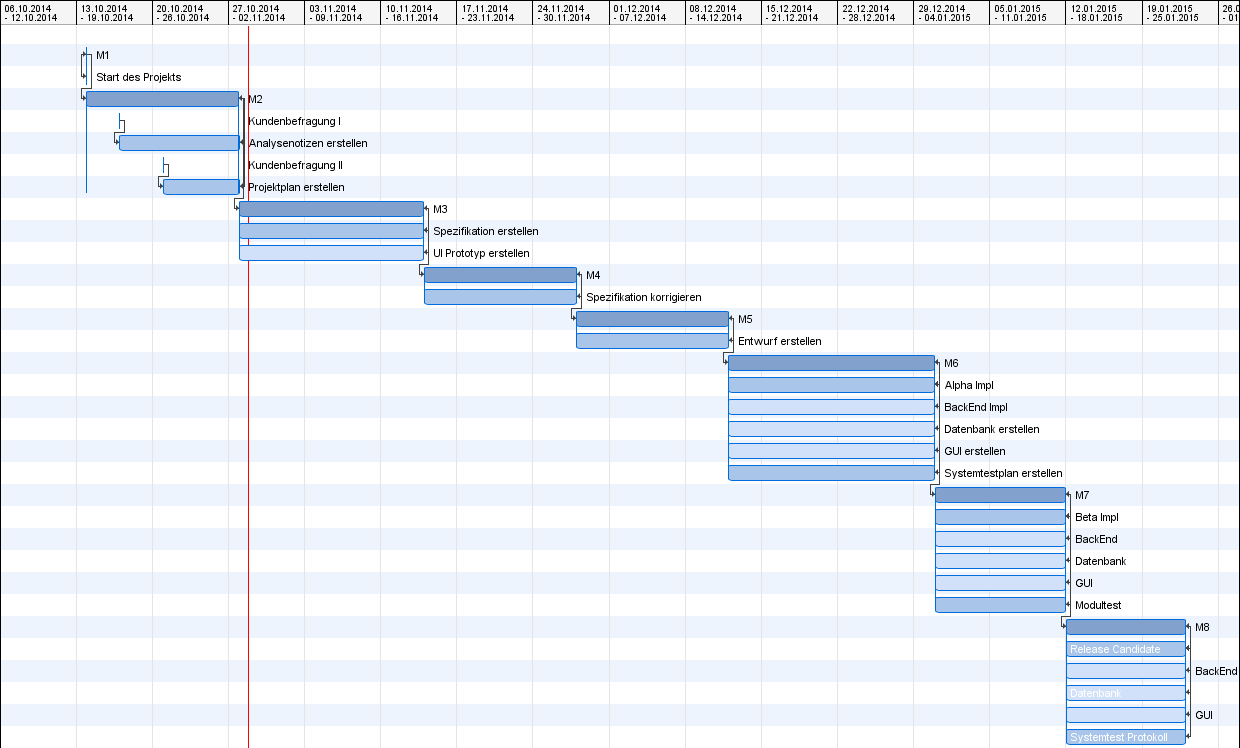
\includegraphics[width=1.0\textwidth]{Gantt.png}
\end{center}

\subsubsection{Termindrift-Diagramm}

\begin{center}
	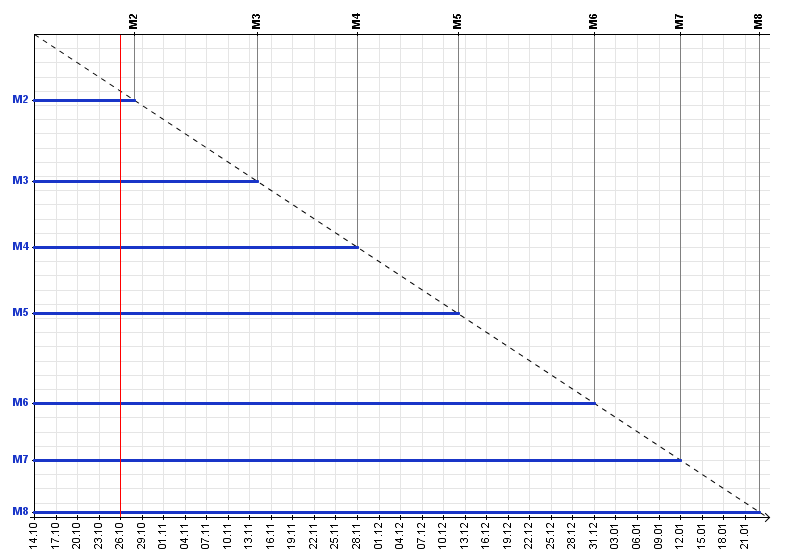
\includegraphics[width=1.1\textwidth]{TerminDrift.png}
\end{center}

\newpage

\section{Risiken}

\subsection{Risiken und ihre Bewertung}

\begin{enumerate}
	\item \textbf{Personenausfall}\\
	\\
	\vbox{\hfill\parbox{14.5cm}{
		\textbf{Risiko}: Hoch\\
		Es kann nicht ausgeschlossen werden, dass Gruppenmitglieder krankheitsbedingt ausfallen.\\
		Außerdem wäre denkbar, dass sich ein Mitglied dazu entschließt das Studium abzubrechen oder in einen anderen Studiengang zu wechseln, was zu permanenten Ausfall führen würde. Dieses Risiko wird aber als sehr unwahrscheinlich eingeschätzt.
	}}
	\\
	\item \textbf{Falsche Funktionalität wird entwickelt}\\
	\\
	\vbox{\hfill\parbox{14.5cm}{
		\textbf{Risiko}: Hoch\\
		Es ist durchaus wahrscheinlich, dass sich die Vorstellungen und Erwartungen an die Funktionalität der Software aus Sicht des Kunden und der der Entwickler unterscheidet. Dies kann dazu führen, dass unnötig Zeit in die Entwicklung von unwichtiger Funktionen fließt und zu wenig Zeit in die Entwicklung von vom Kunden gewünschten Aspekten investiert wird.
	}}
	\\
	\item \textbf{Benutzerschnittstelle entspricht nicht den Vorstellungen des Kunden}:\\
	\\
	\vbox{\hfill\parbox{14.5cm}{
		\textbf{Risiko}: Mittel\\
		Die genauen Vorstellungen des Kunden an die Benutzerschnittstelle des Programms sind schwer in Worte zu fassen. Es besteht keine Möglichkeit über sämtliche Aspekte der Bedienung mit dem Kunden Rücksprache zu halten.
	}}
	\\
	\item \textbf{Termin kann nicht eingehalten werden}\\
	\\
	\vbox{\hfill\parbox{14.5cm}{
		\textbf{Risiko}: Mittel\\
		Fehleinschätzungen von Arbeitsaufwänden und unzureichende Planung kann dazu führen, dass Meilensteine und andere wichtige Termine nicht eingehalten werden können.
	}}
\end{enumerate}

\newpage

\subsection{Gegenmaßnahmen}

\begin{enumerate}
	\item \textbf{Personenausfall}\\
	\\
	\vbox{\hfill\parbox{14.5cm}{
		Da es unmöglich ist dieses Risiko zu eliminieren, müssen entsprechende Vorkehrungen getroffen werden, für den Fall, dass das Risiko eintritt. Dazu zählt eine gute fortlaufende Dokumentation des aktuellen Stands des Projekts, sowie regelmäßige Kommunikation innerhalb des Teams, um den Überblick über das Projekt synchron zu halten und es den übrigen Mitgliedern gegebenenfalls zu ermöglichen, bei einen temporären Ausfall einzuspringen.\\
		Fällt ein Teammitglied dauerhaft aus, muss mit dem Betreuer Rücksprache gehalten werden, um die weiteren Maßnahmen zu besprechen. Zu den denkbaren Maßnahmen zählen insbesondere die Einschränkung des Funktionsumfangs, sowie die Verzögerung von Meilensteinen.
	}}
	\\
	\item \textbf{Falsche Funktionalität wird entwickelt}\\
	\\
	\vbox{\hfill\parbox{14.5cm}{
		Durch die klare Priorisierung der wichtigsten vom Kunden geforderten Funktionalitäten kann dieses Risiko teilweise eingedämmt werden. Die wichtigsten Anforderungen an das Produkt lassen sich entweder aus den von dem Kunden bereitgestellten Dokumenten erschließen, oder wurden in den Kundenbefragungen geklärt. Ein Restrisiko kann alerdings niemals ausgeschlossen werden.
	}}
	\\
	\item \textbf{Benutzerschnittstelle entspricht nicht den Vorstellungen des Kunden}\\
	\\
	\vbox{\hfill\parbox{14.5cm}{
		Laut Anforderungen des Kunden liegt bei der Benutzerschnittstelle der Fokus auf der intuitiven Bedienung des Programms. Es wurden keine konkreten Vorstellungen über Layout oder Design geäußert. Es wird daher angestrebt, die Oberfläche und die Menüführung so simpel wie möglich zu halten, sodass auch Personen ohne entsprechenden Kontext zu der Aufgabe des Programms die Software mit Erfolg bedienen können.\\
		Sollte die Benutzeroberfläche zu stark von den Vorstellungen des Kunden abweichen, muss noch einmal genauere Rücksprache gehalten werden, um die konkreten Kritikpunkte des Kunden abzuändern.
	}}
	\\
	\item \textbf{Termin kann nicht eingehalten werden}\\
	\\
	\vbox{\hfill\parbox{14.5cm}{
		Gerade zum Beginn des Projekts ist es wahrscheinlich, dass der tatsächliche Aufwand des Projekts unterschätzt wird. Das Team wird versuchen den Aufwand so präzise wie möglich einzuschätzen.\\
		Kann ein Termin trotzalledem voraussichtlich nicht eingehalten werden, wird Rücksprache mit den zuständigen Betreuern gehalten. Da die einmalige Verschiebung pro Meilenstein unproblematisch ist, wird gegebenenfalls von dieser Möglichkeit gebrauch gemacht. Anschließend haben Maßnahmen besprochen zu werden, wie und ob der folgende Meilenstein wieder rechtzeitig erreicht werden kann.
	}}
\end{enumerate}

\newpage

\section{Projektorganisation}

\subsection{Ansprechpartner und Beteiligte}

\begin{itemize}
	\item[] \textbf{Kunde}:\\
	\\
	\vbox{\hfill\parbox{14.5cm}{
		Heidelberger Spieleverlag\\
		Dr. August-Stumpf-Strasse 7-9\\
		74731 Walldürn\\
		Deutschland
	}}
	\\
	\item[] \textbf{Team 31}:\\
	\\
	\vbox{\hfill\parbox{14.5cm}{
		Jonas Auer\\
		Matrikelnummer 2860992\\
		\href{mailto:st108421@stud.uni-stuttgart.de}{st108421@stud.uni-stuttgart.de}\\
		
		Fabian Biester\\
		Matrikelnummer 2859084\\
		\href{mailto:st108056@stud.uni-stuttgart.de}{st108056@stud.uni-stuttgart.de}\\
		
		Jan Tagscherer\\
		Matrikelnummer 2893134\\
		\href{mailto:st111459@stud.uni-stuttgart.de}{st111459@stud.uni-stuttgart.de}
	}}
	\\
	\item[] \textbf{Tutor}:\\
	\\
	\vbox{\hfill\parbox{14.5cm}{
		Nicolas Mauch\\
		\href{mailto:nicosurf89@gmail.com}{nicosurf89@gmail.com}
	}}
	
	\newpage
	
	\item[] \textbf{Betreuer}:\\
	\\
	\vbox{\hfill\parbox{14.5cm}{
		Jan-Peter Ostberg\\
		Institut für Softwaretechnologie\\
		Universitätsstraße 38\\
		70569 Stuttgart\\
		Deutschland\\
		\href{mailto:jan-peter.ostberg@informatik.uni-stuttgart.de}{jan-peter.ostberg@informatik.uni-stuttgart.de}\\
		
		Ivan Bogicevic\\
		Institut für Softwaretechnologie\\
		Universitätsstraße 38\\
		70569 Stuttgart\\
		Deutschland\\
		\href{mailto:ivan.bogicevic@informatik.uni-stuttgart.de}{ivan.bogicevic@informatik.uni-stuttgart.de}\\
		
		Wolfgang Fechner\\
		Institut für Softwaretechnologie\\
		Universitätsstraße 38\\
		70569 Stuttgart\\
		Deutschland\\
		\href{mailto:wolfgang.fechner@informatik.uni-stuttgart.de}{wolfgang.fechner@informatik.uni-stuttgart.de}\\
	}}
\end{itemize}

\newpage

\section{Versionshistorie}

\begin{itemize}
	\item Version 1.0 (22.10.2014)
	\begin{itemize}
		\item Grundstruktur des Projektplans erstellt
	\end{itemize}
	\item Version 1.1 (24.10.2014)
	\begin{itemize}
		\item Kapitel 1.1, 1.2, 2.1, 3.1, 5.2 und 5.3 hinzugefügt
	\end{itemize}
	\item Version 1.2 (25.10.2014)
	\begin{itemize}
		\item Kapitel 2.2, 4.1, 4.2, 5.1 und 6.1 hinzugefügt
	\end{itemize}
	\item Version 1.3 (26.10.2014)
	\begin{itemize}
		\item Kapitel 1.3, 4.3, 6.2, 8.1 und 9 hinzugefügt
	\end{itemize}
	\item Version 1.4 (27.10.2014)
	\begin{itemize}
		\item Kapitel 7 hinzugefügt
		\item Gantt- und Termindriftdiagramm hinzugefügt
	\end{itemize}
	\item Version 1.5 (29.10.2014)
	\begin{itemize}
		\item Abkürzungen im Gantt-Diagramm ausgeschrieben
		\item Liste der Beteiligten ergänzt
	\end{itemize}
\end{itemize}

\end{document}
